\documentclass[conference]{IEEEtran}
\IEEEoverridecommandlockouts

\usepackage{amsmath,amssymb,amsfonts}
\usepackage{algorithmic}
\usepackage{graphicx}
\usepackage{textcomp}
\usepackage{xcolor}
\usepackage{tabularx}
\usepackage{cite}
\def\BibTeX{{\rm B\kern-.05em{\sc i\kern-.025em b}\kern-.08em
		T\kern-.1667em\lower.7ex\hbox{E}\kern-.125emX}}
\title{\textbf{Research Design \\}}


\begin{document}

	
	\author{\IEEEauthorblockN{1\textsuperscript{st} Aya Mohamed }
		\IEEEauthorblockA{\textit{Electrical Department} \\
			\textit{Shoubra Faculty of Engineering}\\
		\\
		}

	
		
	}


	\maketitle
%\section{\textbf{Abstract}}
\begin{abstract}
	\label{Section abstract}
	
Research design refers to the method of organization and data collection that a researcher applies to a project or study. If your career involves conducting research, it's crucial to understand the different types of research design that are available for use in your research, So we will discuss in this report What is research design , most  types of it  , The important of it ,The advantage and disadvantage of it .

	
\end{abstract}




\section{\textbf{Introduction}}
\label{section introduction}
A researcher usually chooses the research methodologies and techniques at the start of the research. The document that contains information about the technique, methods and essential details of a project is called a research design\\
Experts define research design as the glue that holds the research project together.\\
It (research design) helps provide a structure and direction to the research, yielding favourable results.\\
 \textbf{Here are some principles of a sound research design:}

\begin{itemize} 
	\item Identifies the problems \\
	\item Reviews literature around the problem statemen \\
	\item Specifies hypothesis \\
	\item Describes sources of data \\
	\item Defines how data will be interpreted \\
		\end{itemize}
 \textbf{ Important concepts of Research Design}
	\begin{itemize}
		
		\item \textbf{Hypothesis} \\
It is defined as the hypothesis that needs to be tested in an experiment\\

		\item \textbf{Independent Variable}\\
An independent variable in an experiment is considered to stand on its own. For instance, if the test scores of a class are an outcome of their efforts; efforts are an independent variable, and the score is a dependent variable\\
		\item \textbf{Dependent Variable}\\
A dependent variable is a variable that is tested in an experiment. It is dependent, in some way on the variation of an independent variable.\\
		\item \textbf{ Variable}\\
Variable is a concept that can take on various quantitative values. For instance, weight, height, etc.e.\\

\end{itemize}
\section{\textbf{Body}}
\textbf{CONCEPT OF RESEARCH DESIGN} \\

Research design provides the glue that holds the research project together. A design is used to 
structure the research, to show how all of the major parts of the research project - the samples or 
groups, measures, treatments or programs, and methods of assignment - work together to try to 
address the central research questions. The function of a research design is to ensure that 
requisite data in accordance with the problem at hand is collected accurately and economically. The
research design, depending upon the needs of the researcher may be a very detailed statement or 
only furnish the minimum information required for planning the research project.\\
\textbf{To be effective, a research design should furnish at least the following details -} .\\
	\begin{itemize}
	
	\item  A statement of objectives of the study or the research output\\

	
	\item  A statement of the data inputs required on the basis of which the research problem is to be 
	solved. \\

	\item  The methods of analysis which shall be used to treat and analyze the data inputs. \\

\end{itemize}
	\begin{figure}[!p!t]
	\centering
	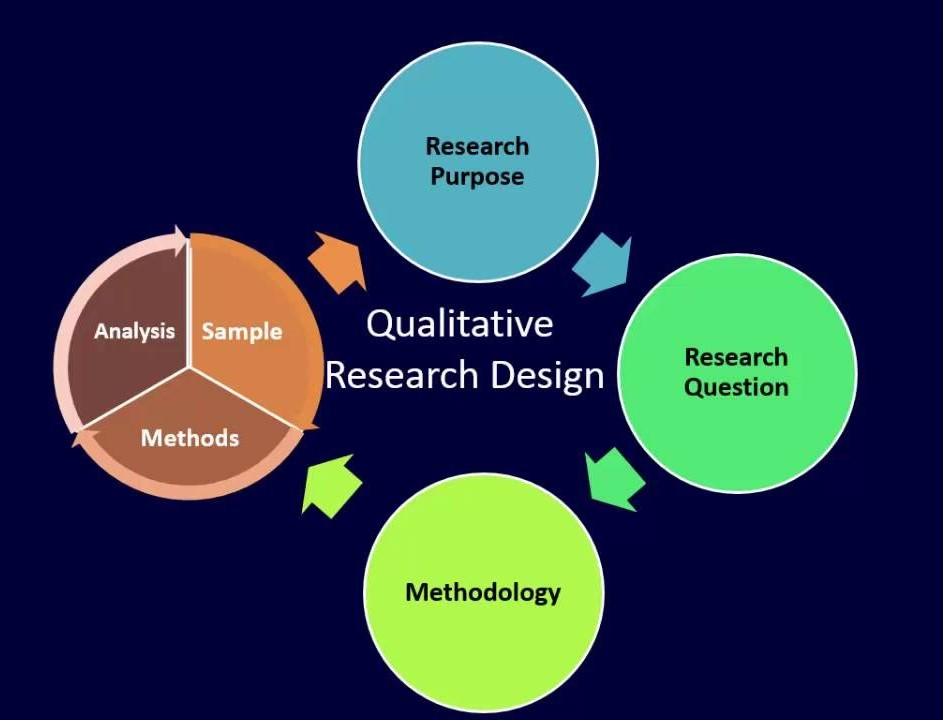
\includegraphics[width=0.5\textwidth]{z}
	\caption{\label{fig:a}}
\end{figure}
 \textbf{the Main Elements of a Research Design}
\begin{itemize}
	
	\item \textbf{Neutrality} \\
	At the start of every research, a researcher needs to make some assumptions that will be tested during the research.
	A proper research design ensures that the assumptions are free of bias and neutral. It also provides that the data collected throughout the research is based on the assumptions made at the beginning of the research.\\
	\item \textbf{Generalised}\\
	A good research design draws an outcome that can be applied to a large set of people and is not limited to sample size or the research group\\
	\item \textbf{Validity}\\
	There are many ways to measure the results of research. A good research design helps select the right measuring tools to gauge results according to the research objective\\
		\item \textbf{Reliability}\\
Research design, when done right, can generate similar results every time it is performed. However, yielding similar results is only possible if your research design is reliable.\\
	
\end{itemize}
 \textbf{Here are some of the elements of a good research design:}
 \begin{itemize}
 	
 	\item Purpose statement \\

 	\item Data collection methods \\

 	\item Techniques of data analysis\\
 
 	\item Types of research methodologies \\
 	\item Challenges of the research \\
 	\item Prerequisites required for study \\
 	\item Duration of the research study \\
 	\item Measurement of analysis \\
 	
 
 	
 \end{itemize}
 
\textbf{What is the need for Research Design?}
\begin{itemize}

	
		\item Reduces inaccuracy\\
		\item  Provides a direction to the research\\
		\item Helpful in testing the hypothesis\\
		\item Minimises wastage of time\\
		\item Eliminates bias and errors\\
		\item Increases efficiency and reliability\\
			
	



\end{itemize}

 \textbf{The most Different Types of Research Design}
\begin{itemize}

	\item \textbf{Quantitative research design}
	Quantitative research design aims at finding answers to who, what, where, how, and when through the course of research. Moreover, the outcome of the quantitative analysis is easy to represent in the form of statistics, graphs, charts, and numbers
	\item \textbf{Qualitative research design}
	Qualitative research design focuses on finding answers to how and why. It uses open-ended questions and helps the subjects express their views clearly.
	Qualitative research is ideal for businesses that aim to understand customers’ behaviour and requirements.
	You can further break the types of research designs into five categories
	\item \textbf{Experimental design}
	This type of research design looks at a problem scientifically by establishing a clear cause and effect of every event. It also tries to understand the impact of the independent variable on the dependable variable.
	Often social sciences use it to observe human behaviours and understand the social psychology of human being better.
	\item \textbf{Correlational design}
	Correlation research design establishes a relationship between two related variables. The researcher observes the variables over time and then draws conclusions based on them. This type of research design requires two different groups.
	A correlation coefficient determines the relationship between two variables. The value of the correlation coefficient ranges between -1 and +1. If the correlation coefficient is +1, it indicates a positive relationship between the two variables, and -1 means a negative relationship
		\item \textbf{Descriptive design}
		Descriptive design is a theory-based research method describing the research’s primary subject matter. This type of research design uses data collection techniques like natural observation, case studies, and surveys to derive results.
		This type of research design provides insight into the why and how of research
			\item \textbf{Diagnostic design}
			In diagnostic research, the design strives to explore the reason behind an issue and find solutions to solve it. This type of research design tries to solve the problems in a structured form divided into three phases- the issue’s inception, diagnosis of the issue, and solution for the issue.
		    \item \textbf{Explanatory design}
				In this research design, the researcher explores concepts and ideas on a subject to explore more theories. The main aim of the research is to explore the subjects’ undiscovered aspects and answer questions like what, how, and why.
				 \item \textbf{Action research design}
				 Another type of research design is the action research design. The action research design format involves initial exploratory analysis and the development of an action strategy. This design format is collaborative, and it focuses on finding solutions, making it practical for many research topics. You can use the action research design when you want to solve real problems.
		\item \textbf{Causal research design}
		The causal research design is another type of research design that researchers commonly choose. The causal research design format attempts to identify and understand relationships between variables, which can be valuable across many industries. Causal research designs typically involve at at least two variables and explore many possible reasons for a relationship between variables.
		\item \textbf{Cohort research design}
		Cohort research design, a type of observational research, is another research design type. This type of research design is commonly used in medicine, but it can also have applications in other industries. Cohort design involves examining research subjects who have already been exposed to a research topic, making it especially effective for conducting ethical research on medical topics or risk factors. This design type is very flexible, and it applies to both primary and secondary data.
			\begin{figure}[!p!t]
			\centering
			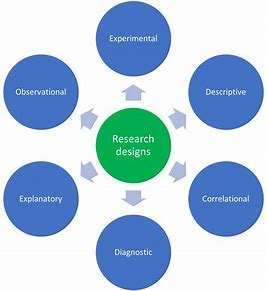
\includegraphics[width=0.5\textwidth]{a}
			\caption{\label{fig:b}}
		\end{figure}
			\item \textbf{Cross-sectional research design}
			Cross-sectional design is another type of observational research design. The cross-sectional research design involves observing multiple individuals at the same point in time. This research type does not alter variables.
				\item \textbf{Sequential research design}
				Sequential research design is another useful type of research design. The sequential research design format divides research into stages, and each stage builds on the last. Therefore, you can complete sequential research at multiple points in time, allowing you to study phenomena that occur over periods of time.
				\item \textbf{Longitudinal research design}
						Another type of quantitative, observational research design is longitudinal design. The longitudinal research design involves observing the same sample repeatedly over a period of time. This time span might be anywhere from a few weeks to several decades, depending on your particular research
				\item \textbf{Mixed-method research design}
				Researchers can also use a mixed-method research design. Mixed-method research designs combine multiple research methods to create the best path for a specific research project. This type of research can include both qualitative and quantitative research methods
			
			
	
	
	

\end{itemize}


\section{\textbf{Methodology }}


\begin{itemize}
	
	\item \textbf{Purpose of Research Design and Methods}
In general, all research serves the purpose of answering questions. The type of question to be answered and the way the answer will be used determine the type of research to be conducted. For example, a fast-food store owner might conduct research to find out which item is a customer favorite, a teacher might conduct research to determine if a particular test is fair, or a government organization might conduct research to determine the need for new community services.
////


Depending on the purpose of the research, the research design and methods may call for reviewing previous research or data (such as in the case of the fast-food store owner), identifying a specific problem (such as in the case of the teacher), or analyzing data (such as in the case of the government agency). Conducting the right research design is important to fit the intended purpose of the research.
\end{itemize}
	\begin{figure}[!p!t]
	\centering
	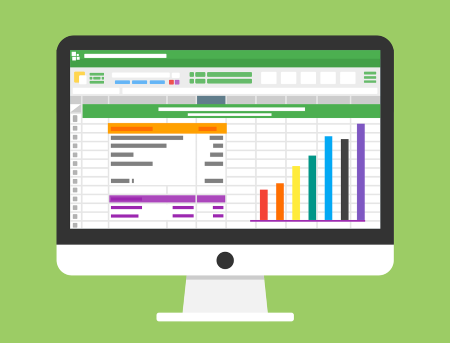
\includegraphics[width=0.5\textwidth]{r}
	\caption{\label{fig:c}}
\end{figure}
\begin{itemize}
	\item \textbf{How to Plan Research Design Methods}
The beginning of a research design is all about planning. When a chef writes a recipe, every step and ingredient must be included to ensure that the recipe can be repeated by others. Similarly, of importance is that researchers plan research designs in a detailed and specific manner and then follow those plans in sequential order so that the research study can be replicated, or repeated with the same results, by others. Replication is an important form of validation for any research project.


In the planning stage of a research design, the researcher must be concerned about three primary steps:
		\begin{itemize}
	\item Data Collection- how data is to be collected (for example, through surveys, qualitative measures, or quantitative measures)
	\item  Measurement- what statistical calculations will be used to evaluate the data.
	\item Analysis- how the statistical measures will be analyzed.

\end{itemize}
\end{itemize}





 


\section{\textbf{Refrenence}}
Jahan, A.K.M.S., Mannan, S.M.,  Kabir, S.M.S. (2013). Designing a Plan for Resource 
Sharing among the Selected Special Libraries in Bangladesh, International Journal of 
Library Science and Research (IJLSR), ISSN 2250-2351, Vol. 3, Issue 3, Aug 2013, 1-20, 
ISSN: 2321-0079\\.
\\
Kabir, S.M.S.  Jahan, I. (2009). Anxiety Level between Mothers of Premature Born Babies 
and Those of Normal Born Babies. The Chittagong University Journal of Biological 
Science, 4(1-2), 131-140.\\
\\
Kabir, S.M.S., Amanullah, A.S.M.,  Karim, S.F. (2008). Self-esteem and Life Satisfaction of 
Public and Private Bank Managers. The Dhaka University Journal of Psychology, 32, 9-
20.\\ 
\\
Kabir, S.M.S., Amanullah, A.S.M., Karim, S.F.,  Shafiqul, I. (2008). Mental Health and Self-esteem: Public Vs. Private University Students in Bangladesh. Journal of Business and 
Technology, 3, 96-108.\\
\\
Kabir, S.M.S., Shahid, S.F.B.,  Karim, S.F. (2007). Personality between Housewives and 
Working Women in Bangladesh. The Dhaka University Journal of Psychology, 31, 73-
84. \\
\\
Kabir, S.M.S. Karim, S.F. (2005). Influence of Type of Bank and Sex on Self-esteem, Life 
Satisfaction and Job Satisfaction. The Dhaka University Journal of Psychology, 29, 41-
52.\\
\\
Kabir, S.M.S.  Rashid, U.K. (2017). Interpersonal Values, Inferiority Complex, and 
Psychological Well-Being of Teenage Students. Jagannath University Journal of Life and 
Earth Sciences, 3(1-2),127-135\\
\\



	






	




\end{document}